\section{Mikrofone}
\label{sec:1}
In dieser Hausaufgabe werden die akustischen Eigenschaften einer Auswahl an Mikrofonen (siehe Tabelle \ref{tab:mics}) analysiert und miteinander verglichen.
Als Grundlage stehen die Frequenzgangsdaten für den Schalldruckpegel aus verschieden Einfallsrichtungen zur Verfügung.

\def\arraystretch{1.5}
\begin{table}[h]
    \centering
    \caption{Auswahl der Mikrofone}
    \label{tab:mics}
    \begin{tabular}{l l l l l}
        Hersteller & Typ & Akustische Arbeitsweise & Richtcharakteristik & Einfallsrichtungen \\
        \hline
        Shure & \texttt{SM58} & Druckgradienten- und Schnelleempfänger & Niere & 0$^\circ$, 90$^\circ$, 180$^\circ$ \\
        Neumann & \texttt{KM120} & Druckgradienten- und Auslenkungsempfänger & Acht & 0$^\circ$, 90$^\circ$, 180$^\circ$ \\
        Neumann & \texttt{KM184} & Druckgradienten- und Auslenkungsempfänger & Niere & 0$^\circ$, 5$^\circ$, ..., 180$^\circ$ 
    \end{tabular}
\end{table}


\subsection{\texttt{K120} und \texttt{SM58} bei Frontalschalleinfall}

Die Abbildung \ref{fig:freq_0} zeigt die auf 1000 Hz normierten Frequenzgänge der Mikrophone bei Frontalschalleinfall.


\begin{figure}[b]
    \centering
    \begin{subfigure}{.5\textwidth}
        \centering
        \caption{KM120}
        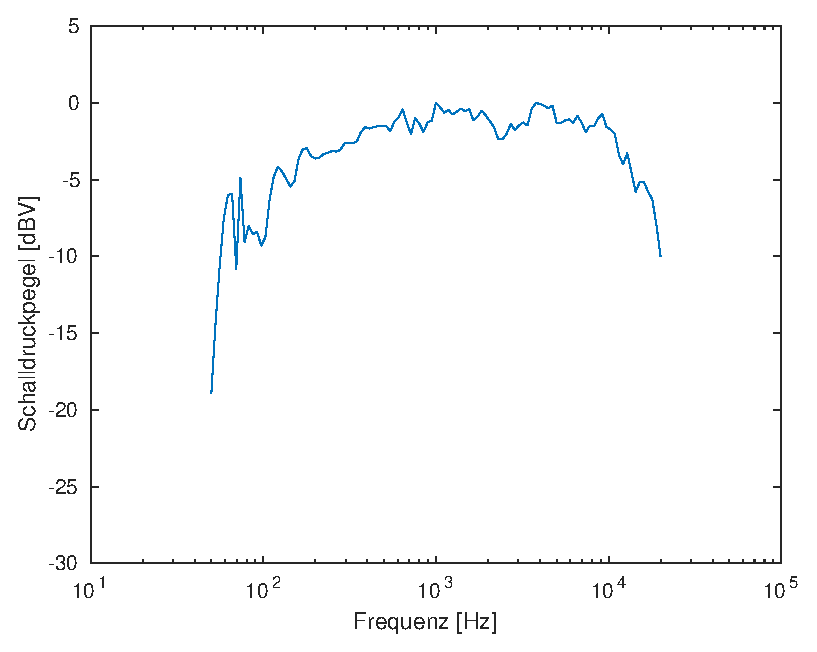
\includegraphics[width=0.95\linewidth]{Figures/km120_0}
    \end{subfigure}%
    \begin{subfigure}{.5\textwidth}
        \centering
        \caption{SM58}
        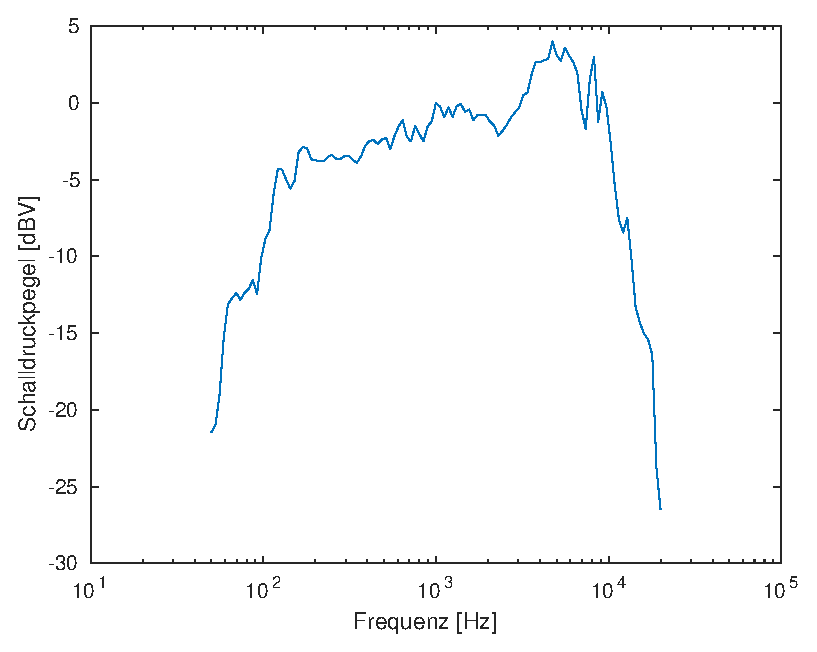
\includegraphics[width=0.95\linewidth]{Figures/sm58_0}
    \end{subfigure}
    \caption{Frequenzgänge der Mikrofone bei Frontalschalleinfall normiert auf 0 dBV bei 1000 Hz}
    \label{fig:freq_0}
\end{figure}

\subsection{Glättung der Frequenzgänge}
Die Implementierung des gleitenden Mittelwerts nehmen wir mit der filter() Methode aus Matlab vor.
Das resultierende geglättete Spektrum ist in Abb. \ref{fig:freq_movmean} zu sehen. Das Verhältnis benachbarter Frequenzbins ist konstant und beträgt $f_{n+1}/f_{n} = 1.057$.
Die Frequenzauflösung der Spektren ist somit nicht linear, sondern abhängig von der Frequenz.
Zudem mittelt der gleitende Mittelwert konstant über drei Bins.
Das bedeutet, dass wir es mit einer Glättung mit relativer Bandbreite zu tun haben.
Allerdings ist es weder eine terzbreite noch eine oktavbreite Glättung.
In beiden Fällen müsste das Frequenzverhältnis benachbarter Bins größer sein.
Allgemein gilt: Eine Glättung mit relativer Bandbreite liefert eine gleichmäßigere Kurve in logarithmischer Darstellung der Frequenzachse des Spektrums, als eine Glättung mit konstanter Bandbreite.
Diese liefert wiederum eine gleichmäßig geglättete Kurve für die Darstellung mit linearer Frequenzachse.

\begin{figure}[b]
    \centering
    \begin{subfigure}{.5\textwidth}
        \centering
        \caption{KM120}
        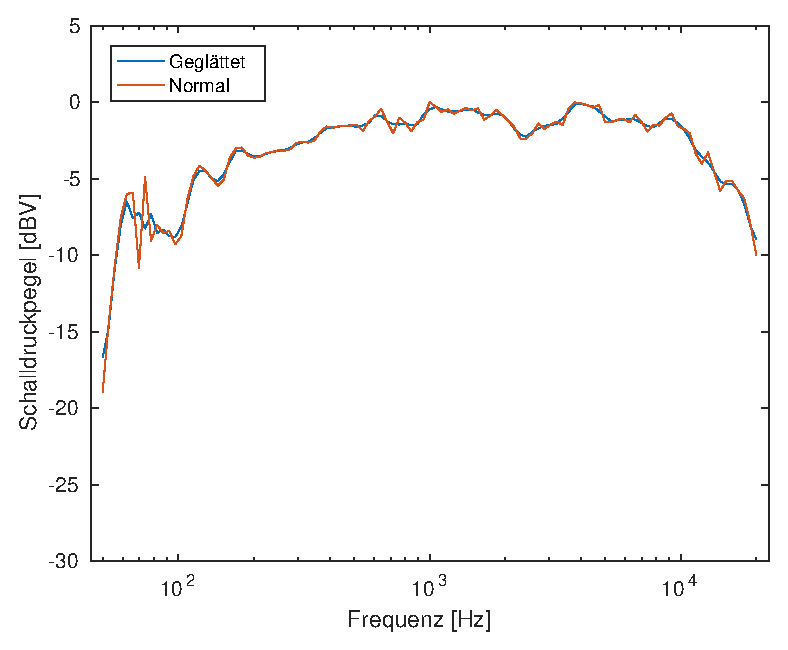
\includegraphics[width=0.95\linewidth]{Figures/km120_0_movmean}
    \end{subfigure}%
    \begin{subfigure}{.5\textwidth}
        \centering
        \caption{SM58}
        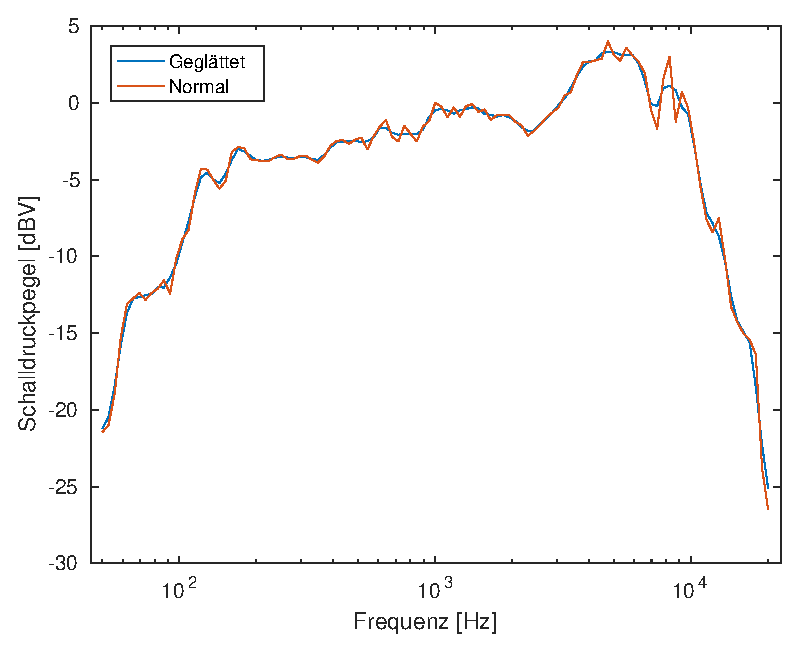
\includegraphics[width=0.95\linewidth]{Figures/sm58_0_movmean}
    \end{subfigure}
    \caption{Unterschied zwischen dem normalen und dem geglätteten Frequenzgang der Mikrofone bei frontalem Schalleinfall}
    \label{fig:freq_movmean}
\end{figure}

\subsection{Weitere Einfallsrichtungen}

Die Abbildung \ref{fig:freq_all} zeigt die bei 0° auf 1000 Hz normierten Frequenzgänge der Mikrophone in 3 unterschiedlichen Einfallsrichtungen.

\begin{figure}[b]
    \centering
    \begin{subfigure}{.5\textwidth}
        \centering
        \caption{KM120}
        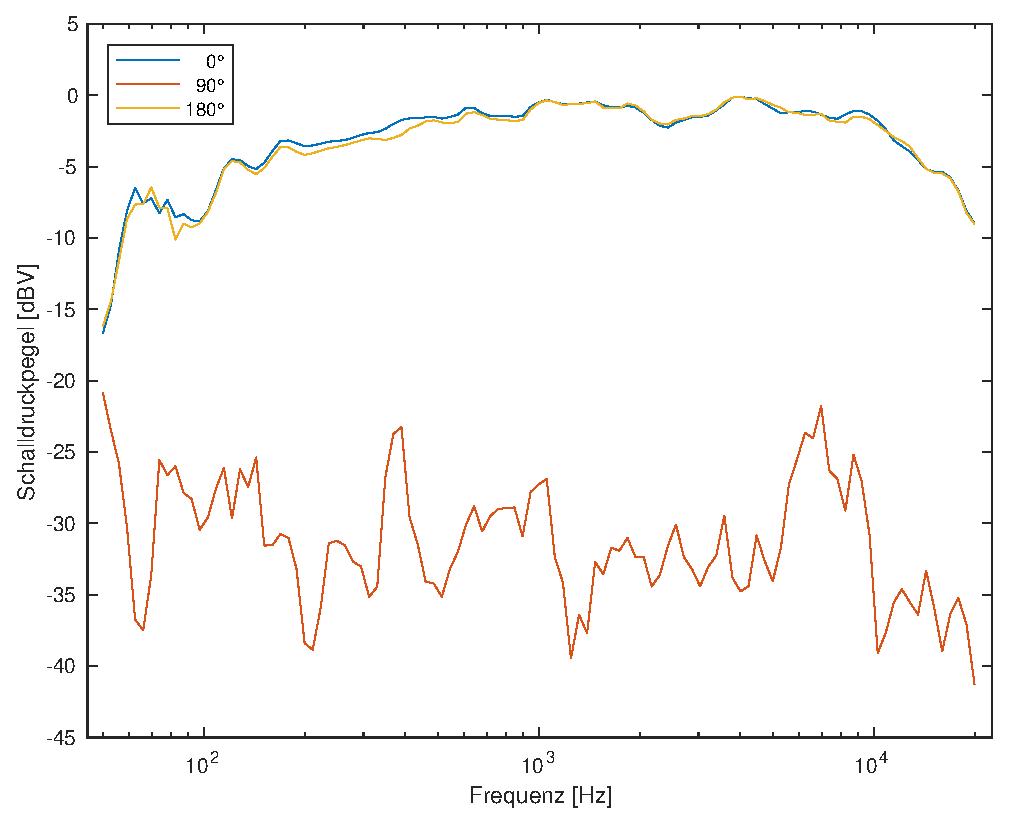
\includegraphics[width=0.95\linewidth]{Figures/km120_all}
    \end{subfigure}%
    \begin{subfigure}{.5\textwidth}
        \centering
        \caption{SM58}
        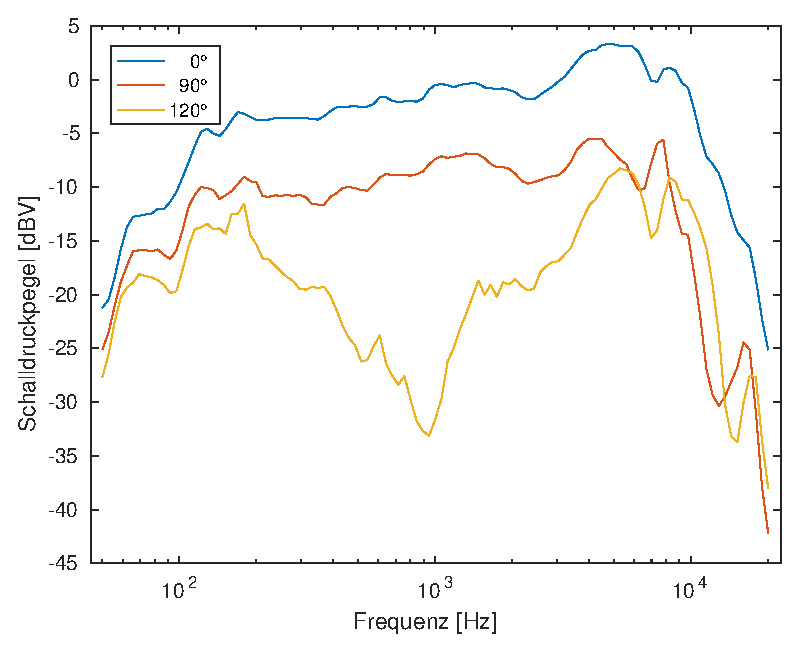
\includegraphics[width=0.95\linewidth]{Figures/sm58_all.eps}
    \end{subfigure}
    \caption{Geglättete Frequenzgänge aus drei verschiedenen Einfallsrichtungen}
    \label{fig:freq_all}
\end{figure}


\subsection{Richtcharakteristik}